\subsection{记录观察时域的影响}
\label{sec:record-ablation}
为考察增加下一事件的作用，在同一攻击策略下改变记录观察时域。沿用S、U系统和目标时刻 $k=4$，
在目标之前不施加攻击，仅在目标发送时实施命题\ref{prop:deletion}的一步保分布MH修改，
之后不再攻击。其提议步长为 $\pm b{\bm{v}}$，拒绝时保持原载荷，故逐路径满足同一峰值限制。
详细平衡使截至目标时刻的完整日志 $H_k$ 与无攻击运行严格同律；
这一等式由解析构造保证。

该策略的损伤、统计损伤证书及记录分布差异如图\ref{fig:record-ablation}所示。
当 $b=0.1$ 时，S、U中的损伤分别约为 $2.995\times10^{-4}$ 和 $5.360\times10^{-4}$，
而扩展事件串 $\gamma_{0:k+1}$ 的TV分别约为 $6.401\times10^{-5}$ 和 $1.609\times10^{-4}$。
加权下一静默事件给出的统计损伤证书分别约为 $4.258\times10^{-4}$ 和 $8.430\times10^{-4}$。
可见，截至目标时刻的日志同律仍伴随正损伤；记录增加下一事件后，预测偏差使静默概率发生变化，从而得到损伤上界。
这里的证书与真实损伤之差反映该固定策略下的保守性，与图\ref{fig:vector-budget}中的全策略最坏损伤界属于不同的比较。

本例各历史下的下一静默概率变化同号，末事件位TV恰等于扩展事件串TV。
该工况据此验证了延长观察时域的作用，但没有体现历史标记相对于末事件位的优势。
历史信息缺失时可能出现的概率抵消由命题\ref{prop:last-bit}给出。
图中统计损伤证书采用总体概率，不含有限样本余量；有限样本置信上界见附录\ref{app:statistical}。
事件串TV也仅为完整扩展日志TV的下界。
接受质量积分、误差诊断及复现步骤见附录\ref{app:record-ablation}。

\begin{ecustfigure}
\centering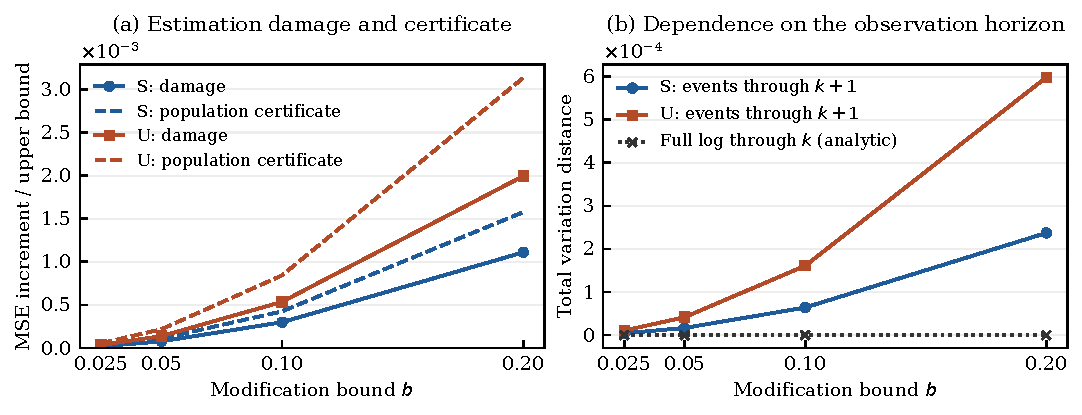
\includegraphics[width=.96\textwidth]{figures/record_conditions.pdf}
\figcaption{同一当拍保分布攻击下的损伤与记录时域对照：截止日志TV为解析零值，扩展事件TV为浮点求积结果}{Damage and record horizons under the same distribution-preserving attack: cutoff-log TV is analytically zero; extended-event TV is evaluated by floating-point quadrature}
\label{fig:record-ablation}
\end{ecustfigure}

